\chapter{固体与流体}

\textcolor{red}{\textbf{\textit{/大学物理I“流体力学入门”内容/}}}
\hfill{\textcolor{blue}{\textit{by HuSP，欢迎加入}}}%画矢量图？来个GitHub？

\begin{introduction}
    \item 应力与应变
    \item 静止流体的压强
    \item 理想流体的稳定流动
    \item 伯努利方程
    \item 粘滞流体的运动
    \end{introduction}

\section{应力与应变}    %\label{?.1}
\subsection{Pre-}
固体:能保持其体积和形状的物质;

液体:能保持其体积但不能保持其形状的物质;

气体:既不能保持其体积也不能保持其形状的物质。

流体：气体、液体；

基本特性：没有固定的形状，具有流动性。

连续介质模型：将流体看成由无限多流体质点组成的稠密而无间隙的连续介质。

\subsection{应力}
作用于物体的应力产生应变

当 $\sum \vec{F}_{i}=0 \quad \sum \vec{M}_{i}=0$ 时,

\begin{equation}
	\sigma=F/S
\end{equation}

具体情况有如下几种
\begin{center}
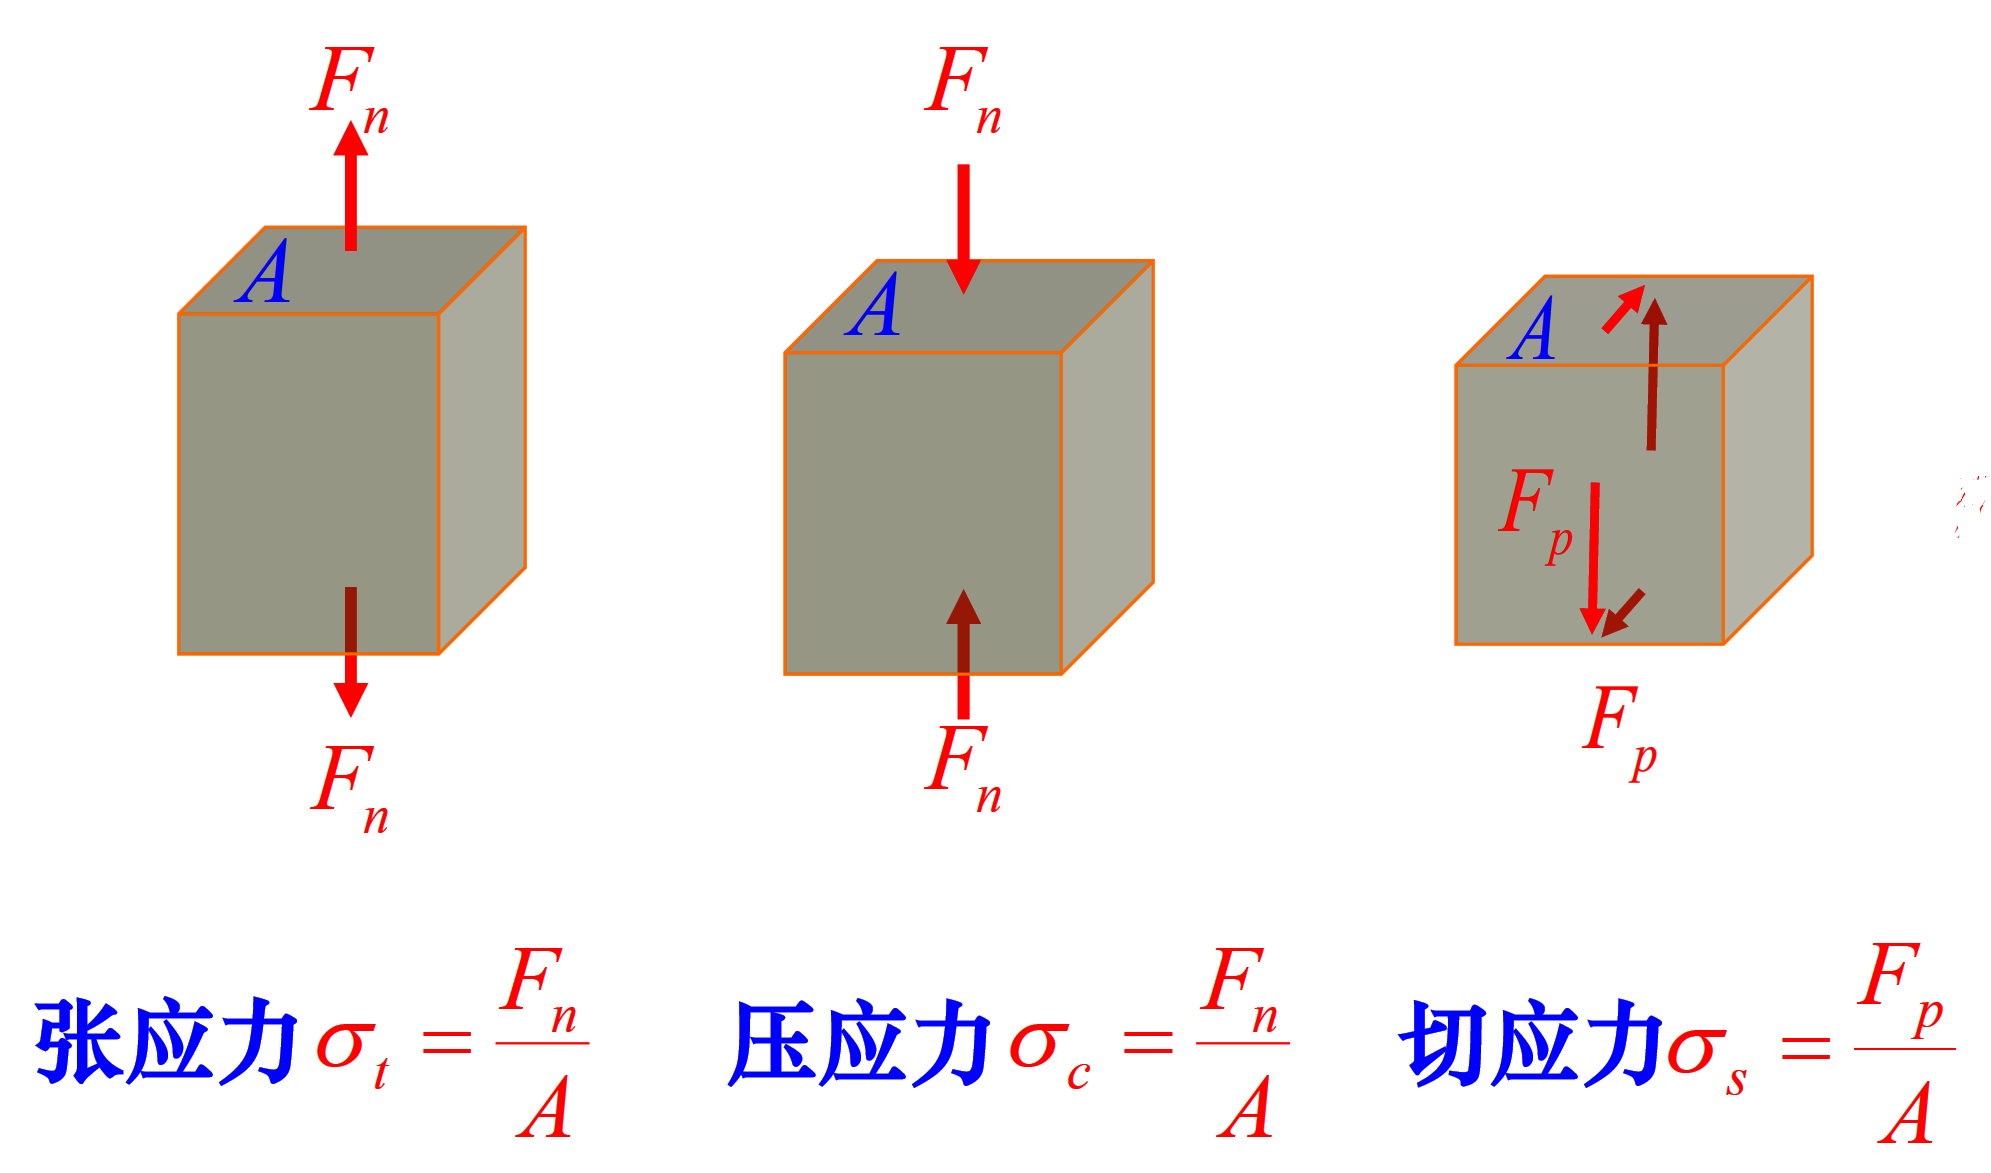
\includegraphics[scale=0.2]{Cf-pic (1).png}
\end{center}
注意:与物体受到各方向的压力所产生的压强区分(A是正压力对应面积)
\begin{equation}
	p=\frac{F_{n}}{A}
\end{equation}

\subsection{应变}
物体受应力作用时产生变形的量度。同理，分类如下：
\begin{center}
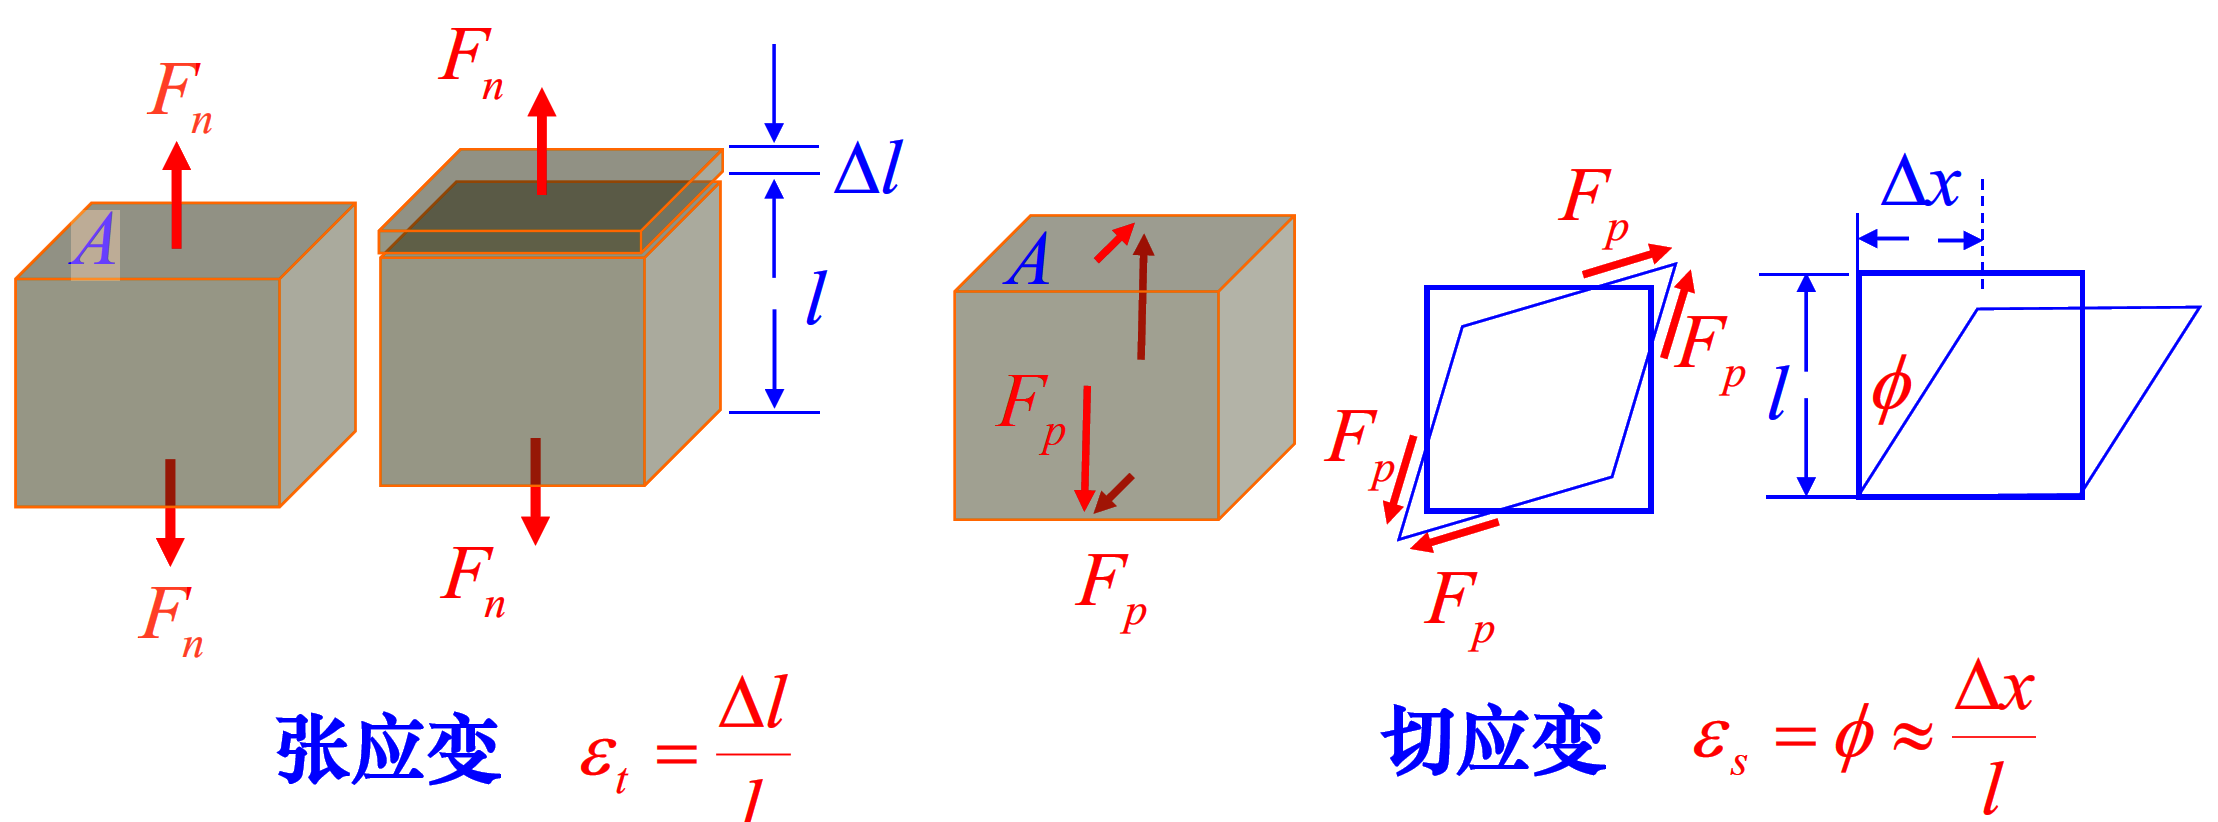
\includegraphics[scale=0.22]{Cf-pic (2).png}
\end{center}

\subsection{关系（模量）}
应力$\propto$形变. 从“弹性模量”可以得出固体、液体、气体的性质。

如杨氏（弹性）模量Y，切向模量S，体积模量B：
\begin{equation}
	Y=\frac{\sigma_{t}}{\varepsilon_{t}}=\frac{F_{n} / A}{\Delta l / l} \qquad S=\frac{\sigma_{s}}{\varepsilon_{s}}=\frac{F_{p} / A}{\Delta x / l} \qquad    B=-V \frac{\mathrm{d} p}{\mathrm{~d} V} \approx-\frac{\Delta p}{\Delta V / V}
\end{equation}

\section{静止流体中的压强}

在静止的流体中不可能存在切应力 。\\
——在限制流体的所有表面上,力必然垂直于表面。\\
——与作用面取向无关。
\vskip 0.5cm
由此，基于流体元作受力分析：
\begin{enumerate}
	\item 等高点压强：$P_A=P_B$
         \\(由受力分析$P_A⋅\Delta s- P_B⋅\Delta s = Δma_x$得，可推广至稳恒匀速流动)
	\item 高度相差h两点的压强差：(此处强调不可压缩)
         \\沿y方向$a_y=0$,而$P_{B} \cdot \Delta s-P_{C} \cdot \Delta s-\Delta m g=\Delta m a_y \Rightarrow P_{BC}=\rho gh$
    \item （由上，）帕斯卡原理的应用：
        \begin{center}
        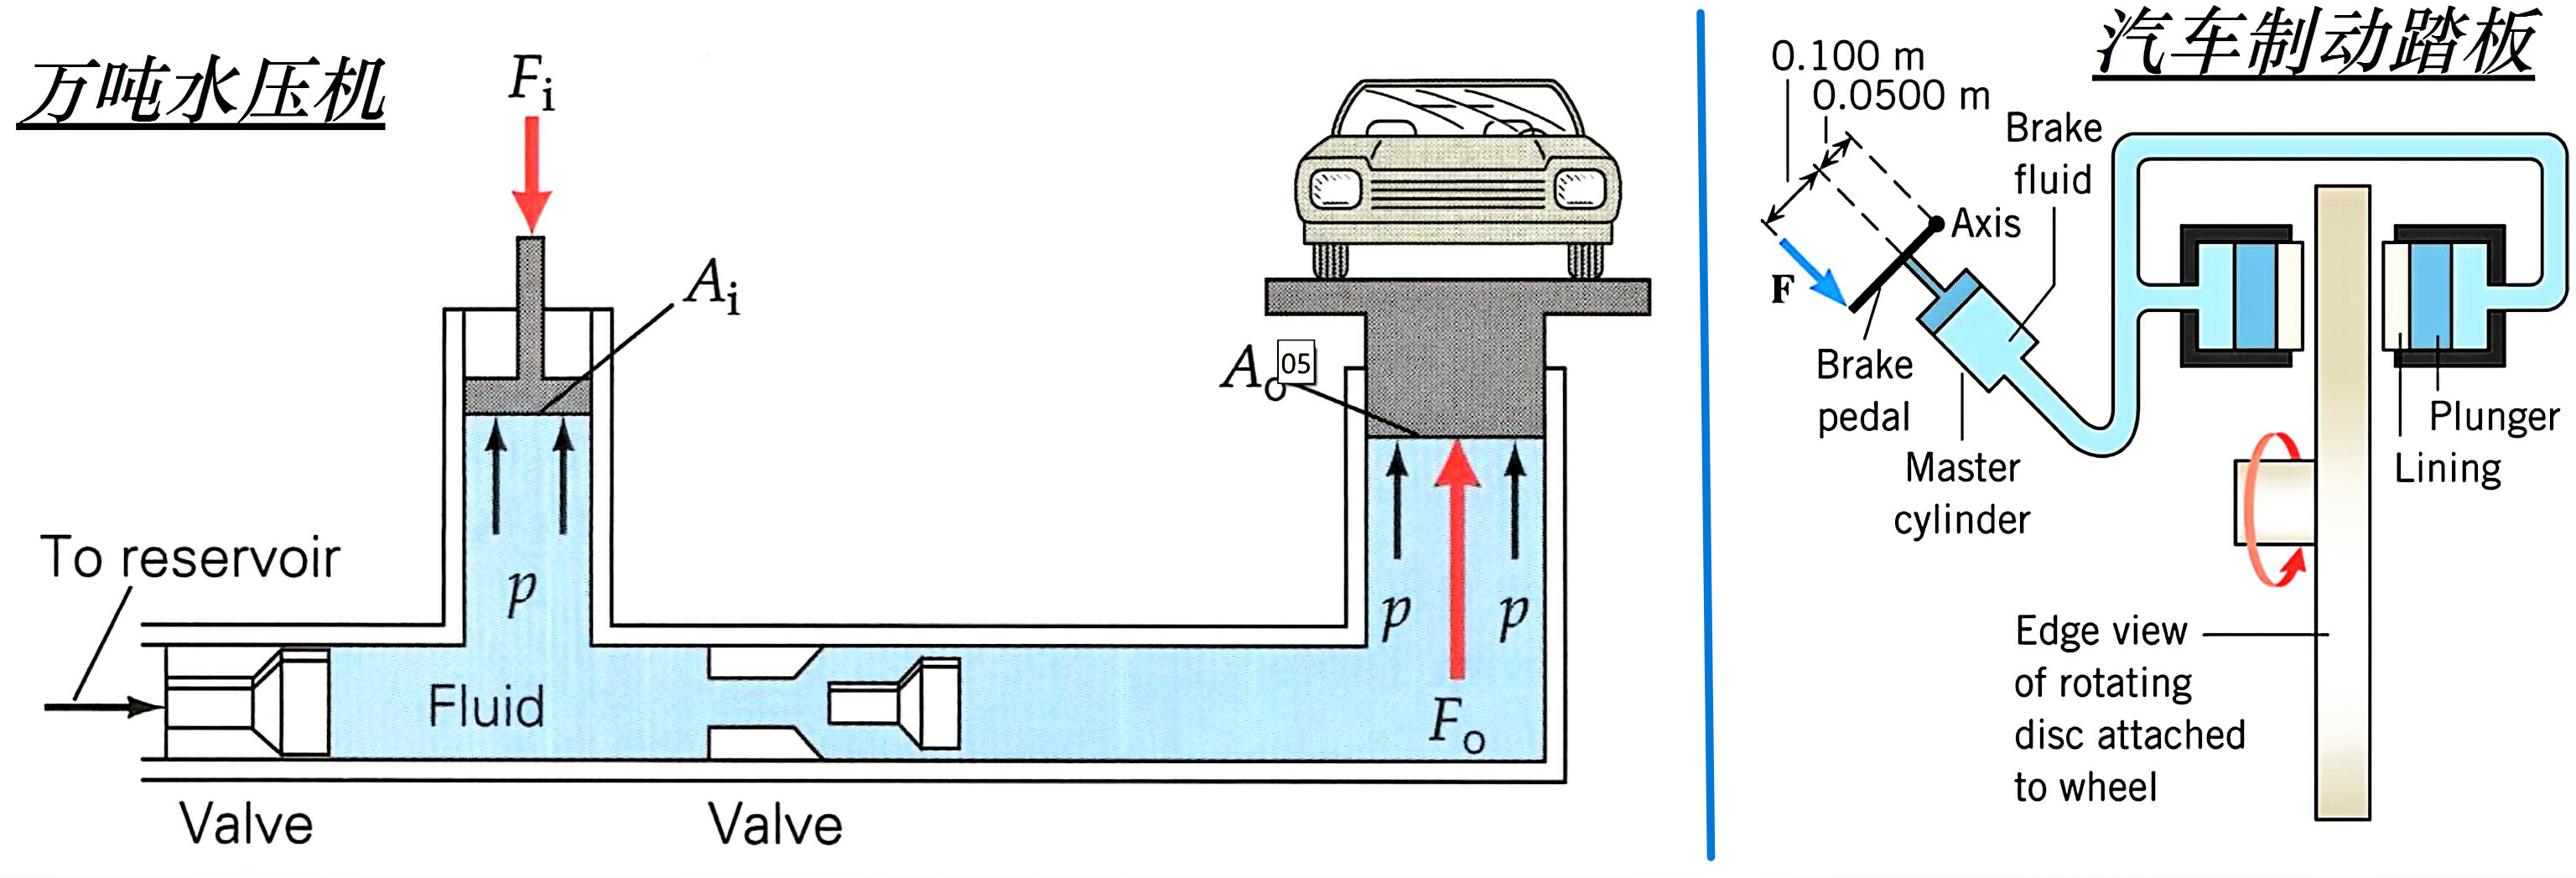
\includegraphics[scale=0.13]{Cf-pic (3).png}
        \end{center}
        AND，一个水桶绕自身的竖直轴以角速度ω旋转，当水与桶一起转动时，水面的形状是 \textbf{抛物面} 。
    \item 可压缩流体高度相差h两点的压强差：（如气体）
        \\\begin{equation}
	    d p=-p g d y
         \end{equation}\begin{equation}
         p V=\frac{m}{M_{\mathrm{mol}}} R T \Rightarrow p=\frac{1}{M_{\mathrm{mol}}} \rho R T
         \end{equation}\begin{equation}
         \mathrm{d} p=-\frac{\rho_{0}}{p_{0}} p g \mathrm{~d} y \quad \frac{\mathrm{d} p}{p}=-\frac{\rho_{0}}{p_{0}} g \mathrm{~d} y
         \end{equation}\begin{equation}
         \int_{p_{0}}^{p} \frac{\mathrm{d} p}{p}=-\int_{0}^{y} \frac{\rho_{0}}{p_{0}} g \mathrm{~d} y 
          \end{equation}\begin{equation}
          \Rightarrow p=p_{0} e^{-\left(\rho_{0} g / p_{0}\right) y}
         \end{equation}
         最后的结果被称为 \textit{等温气压公式} 。由此有 \textit{阿基米德原理} ，产生浮力。
\end{enumerate}

\section{理想流体的稳定流动}

\subsection{理想流体}
不可压缩的无黏滞性的流体称为理想流体（\textcolor{red}{\textbf{理想模型}}）
\begin{enumerate}
	\item 压缩性
     \begin{itemize}
         \item 流体受压缩时其密度变化可忽略时，可看作不可压缩流体；
         \item 液体压缩性小($\rho=$常量);
         \item 气体压缩性大，流动性也大。
     \end{itemize}
	\item 粘滞性
     \begin{itemize}
         \item 流体在流动时，若能量损耗可忽略 ，可看作非黏滞流体；
         \item 气体和某些液体（如：水）黏滞性小，可以忽略；
         \item 无粘滞性流体运动过程中没有切向相互作用，受力具有静止流体的特征。即，有粘滞性流体中各点的速度不同。
         \begin{center}
        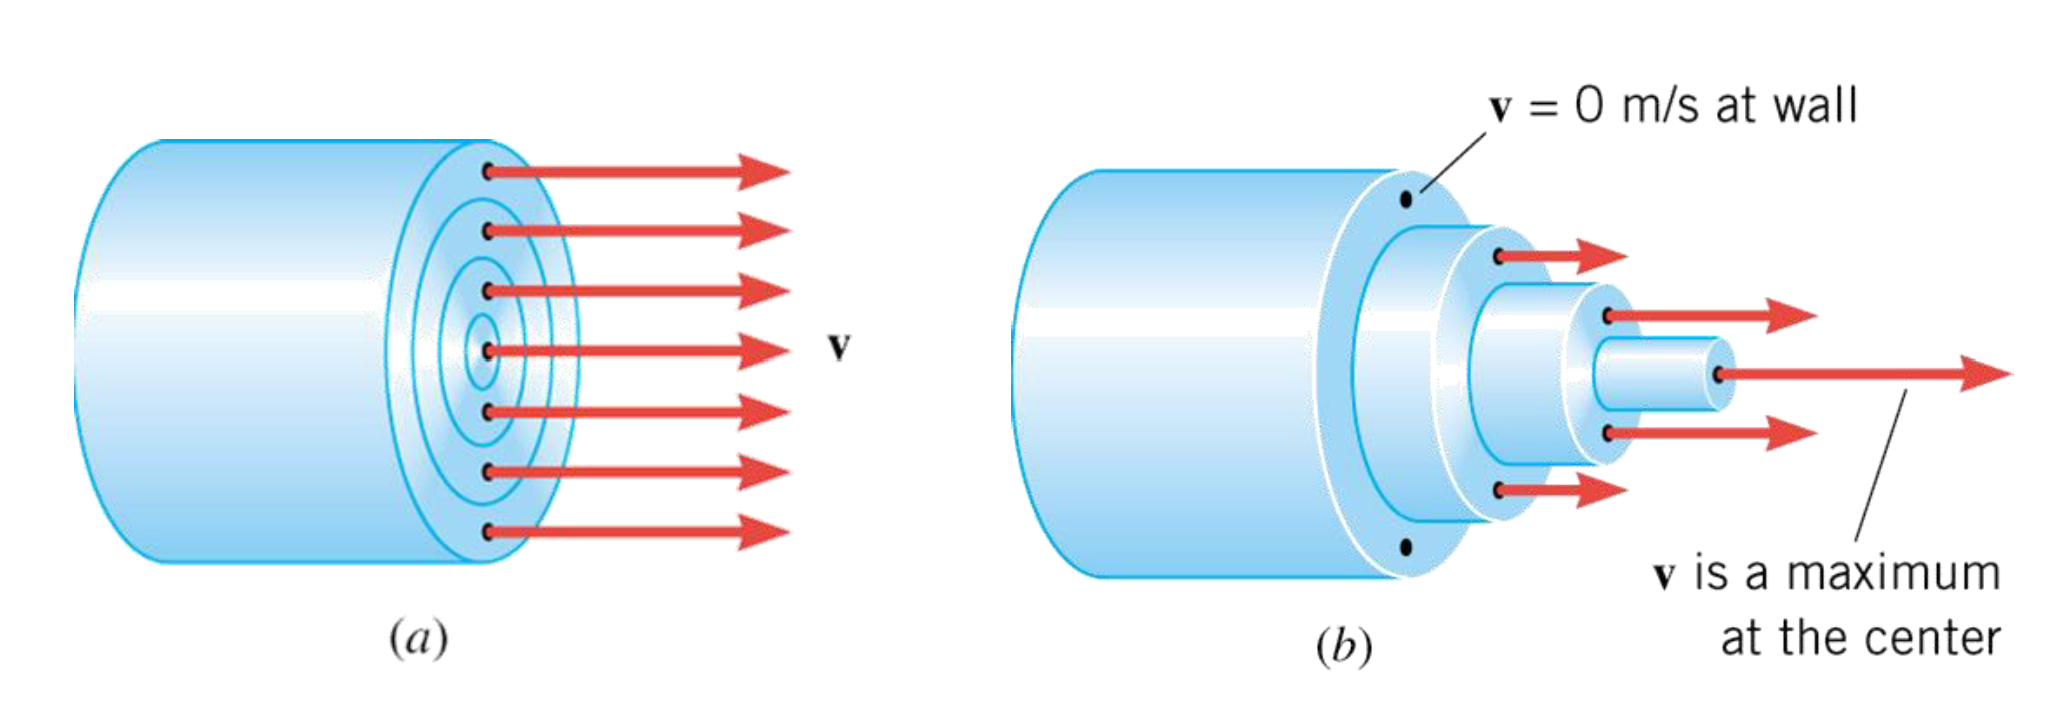
\includegraphics[scale=0.55]{Cf-pic (4).png}
        \end{center}
        流体的黏滞性 取决于流体内部接触层间切向黏滞力 (内摩擦力) 的大小。
     \end{itemize}
\end{enumerate}

\subsection{流体的稳定流动}
\begin{enumerate}
	\item 流速场：描述流体中流体质点速度的分布
        \begin{equation}
	    \overrightarrow {\rm{v}}  = \overrightarrow {\rm{v}} \left( {x,y,z,t} \right)
        \end{equation}
        稳定流动时：\textbf{与t无关}
    \item 流线（类比电场线）\\
        /连续/不可相交/流线与时刻相对应[而非轨迹]/
    \item 流管：由流线围成的管状区域\\
        流管外的流体不会流入流管，内部的也不会流出——质量守恒。
\end{enumerate}

\subsection{流量}
单位时间内流过面积S的流体\textbf{体积或质量}。\hfill(PS. 通量：$\[\Phi  = \int_{\rm{S}} {\overrightarrow {\rm{A}}  \cdot d{\rm{S}}} \]$)

\subsection{理想流体的连续性方程}
在稳定流动的流体中取一细流管（S1、S2为垂直流线的两个截面）(理想流体 $\rho_1=\rho_2$)，有
\begin{equation}
	v_1 S_1 =v_2 S_2
\end{equation}
值得说明的是：
\begin{enumerate}
	\item 连续性方程是质量守恒定律的必然结果；
    \item 例子：水龙头刚流出的水柱（湍流区前）；
    \item 流速较大的地方流线密；
    \item 细流管：\textbf{物理上的“细”指截面上各处速度一样，不论大小}；
    \item $\Rightarrow$ 环路面积分为0
\end{enumerate}

\section{伯努利方程}

\subsection{伯努利方程（1726）}

\textit{丹尼尔·伯努利(1700-1782)把牛顿力学引入对流体的研究,也是气体动力学专家。}
伯努利方程理想流体在重力场中的稳定流动——

取一细管ab从$a_1$$b_1$运动到$a_2$$b_2$，可视为$a_2$$b_1$不动而$a_1$$a_2$部分运动到$b_1$$b_2$处。

\begin{center}
        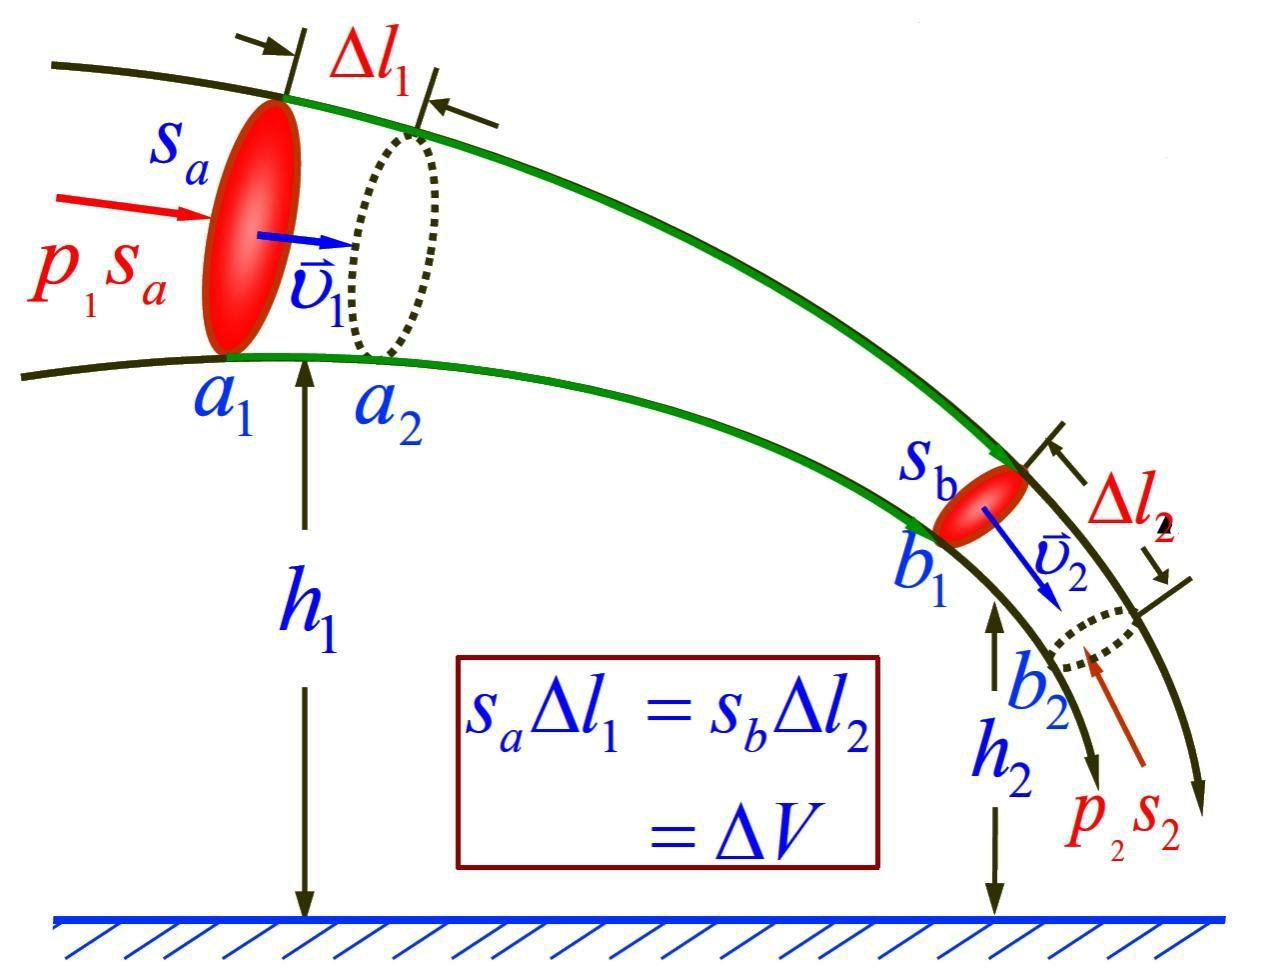
\includegraphics[scale=0.2]{Cf-pic (5).png}
\end{center}

研究对象：地球+ab部分流体

故，内好的功为零的情况下，由功能原理：
\begin{equation}
	    A_外=p_1s_a·\Delta l_1-p_2s_b·\Delta l_2=(p_1-p_2)\Delta V  ==  \Delta E_k+\Delta E_p=...
\end{equation}
展开两能量增量并移项，可得出伯努利方程：同一流管中，任一点处流体单位体积的动能和势能以及该处压强之和为常量
\begin{equation}
	p_1+\rho gh_1+\frac{1}{2}\rho v_1^2=p_2+\rho gh_2+\frac{1}{2}\rho v_2^2=···=Const
\end{equation}
值得说明的是：
\begin{enumerate}
	\item 伯努利方程是能量守恒定律在流体力学中的应用。
    \item 适用于理想流体的稳定流动。
    \item 各物理量均为国际单位
    \item 静止流体：$p_2-p_1=\rho g(h_1-h_2)$
    \item 水平流管：
        \begin{equation}
	        p_1+\frac{1}{2}\rho v_1^2=p_2+\frac{1}{2}\rho v_2^2
        \end{equation}
        \textbf{推论：}同一水平流管中，任一截面处，压强相等则流速必相等；流速大处则压强小；流速小处则压强大。
        
        \textbf{应用：}船吸现象、足球香蕉球\footnote{马格努斯效应}、飞机机翼、屋顶、火车站台…
\end{enumerate}

\subsection{伯努利方程的应用}
\subsubsection{小孔泄流问题}
在大容器的器壁上水深为h处，开一小圆孔，不计任何阻力。
分别以液面处和小孔处为研究对象：

由伯努利方程：
\begin{equation}
	p_A+\rho gh+\frac{1}{2}\rho v_A^2=p_2+\frac{1}{2}\rho v_B^2
\end{equation}
考虑到 \quad $v_A\approx 0 ,\qquad p_A=p_B=p_0$
\begin{equation}
	v=\sqrt{2gh} \qquad\footnote{又称托里拆利公式}
\end{equation}
即，流体从小孔流出的速度与流体质点由液面处自由下落到小孔处的速度大小相等。

还可拓展为 \textbf{虹吸管}，只将下端管口与液面的高度差（当然液面需高于管口）替换h，执行上式即可。

\subsubsection{皮托管}
用于测量流体流速。1979年皮托用此测出了塞纳河的流速，后改进可测气体(如图，推导略去)。
\begin{center}
        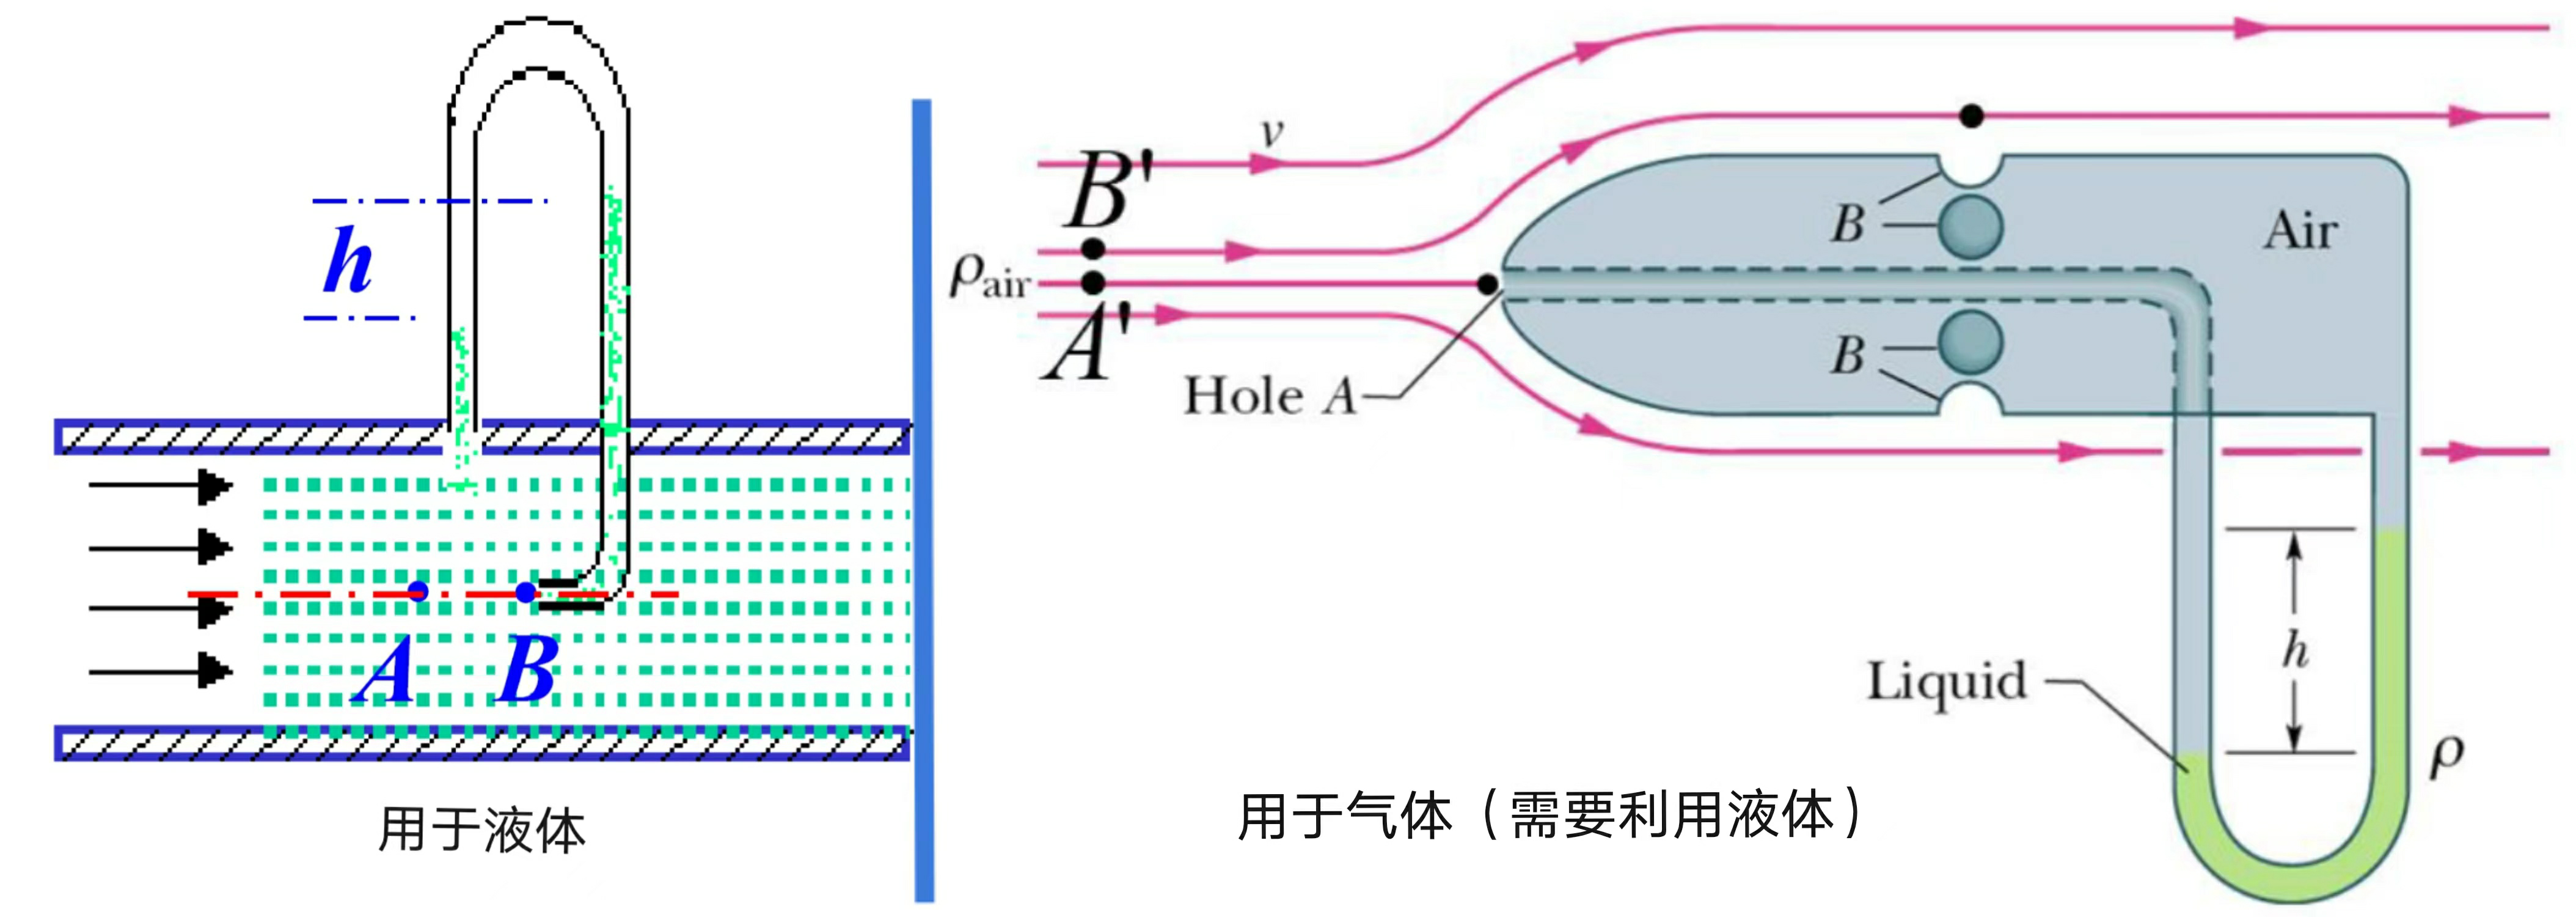
\includegraphics[scale=0.11]{Cf-pic (6).png}
\end{center}
设液面高度差为h，
则对液体测量装置：
\begin{equation}
	v=\sqrt{2gh}
\end{equation}
对气体流速测量装置：由$p_A=p_B+\rho gh$，有
\begin{equation}
	v=\sqrt{2gh·\frac{\rho}{\rho^{\prime}}} 
\end{equation}

\subsubsection{文特利流量计与空吸作用}
文特利流量计（从原型开始）
\begin{center}
    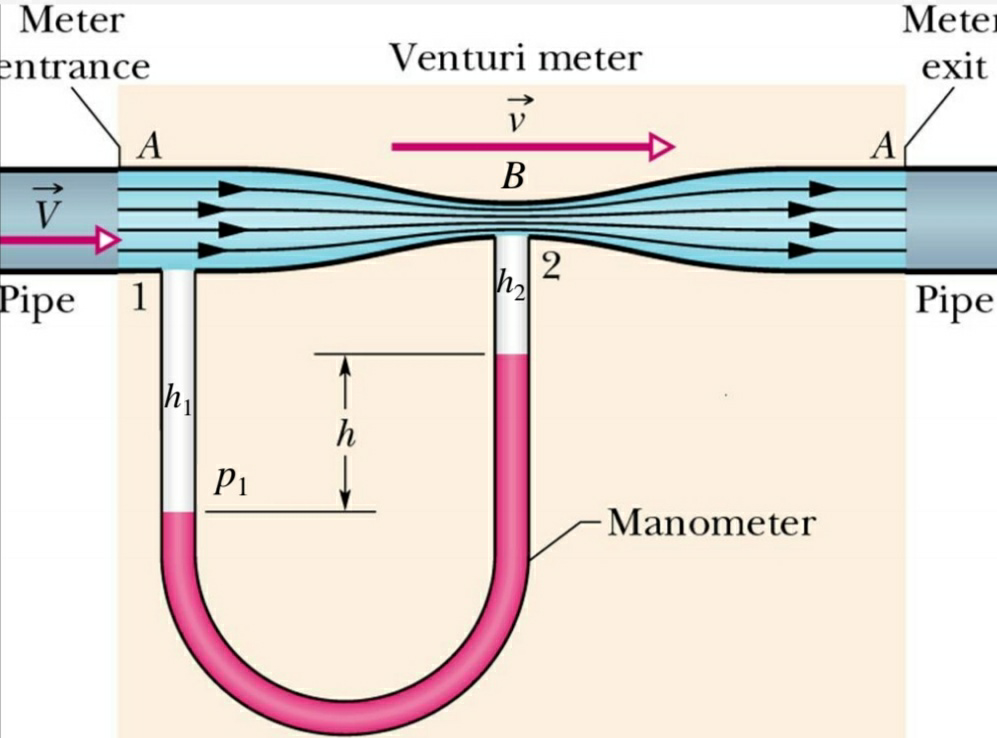
\includegraphics[scale=0.2]{Cf-pic (7).png}
\end{center}

\begin{equation}
	p_A+\frac{1}{2}\rho v_A^2=p_B+\frac{1}{2}\rho v_B^2 \qquad v_AS_A=v_BS_B
\end{equation}
\begin{equation}
    \Rightarrow\left\{\begin{array}{l}v_{A}=\sqrt{\frac{2\left(p_{B}-p_{A}\right)}{\rho\left(S_{B}^{2}-S_{A}^{2}\right)}} S_{B} \\ v_{B}=\sqrt{\frac{2\left(p_{A}-p_{B}\right)}{\rho\left(S_{A}^{2}-S_{B}^{2}\right)}} S_{A}\end{array}\right.
\end{equation}    
\begin{equation}
    Q_V=v_AS_A=\sqrt{\frac{2\left(p_{A}-p_{B}\right)}{\rho\left(S_{A}^{2}-S_{B}^{2}\right)}} S_{A} S_{B}=\sqrt{\frac{2\left(\rho_{\text {汞 }}-\rho\right) g h}{\rho\left(S_{A}{ }^{2}-S_{B}{ }^{2}\right)}} S_{A} S_{B}
\end{equation}
\begin{multicols}{2}
~\\
而在现代装置中，还可以纵置：
~\\
    \begin{equation}
        p_1+\rho gd+\frac{1}{2}\rho v_1^2=p_2+\frac{1}{2}\rho v_2^2
    \end{equation}
    \begin{equation}
        v_1S_1=v_2S_2
    \end{equation}
    结果是，
    \begin{equation}
        Q_{V}=\sqrt{\frac{2\left(p_{1}-p_{2}+\rho g d\right)}{\rho\left(S_{1}^{2}-S_{2}^{2}\right)}} S_{2}
    \end{equation}
    ~\\
    \begin{equation}
        v_{1}=\sqrt{\frac{2\left(p_{1}-p_{2}+\rho g d\right)}{\rho\left(S_{1}^{2}-S_{2}^{2}\right)}} S_{1} S_{2}
    \end{equation} 
    ~\\
    （横置只需令$\rho gh=0$）
    \begin{center}
        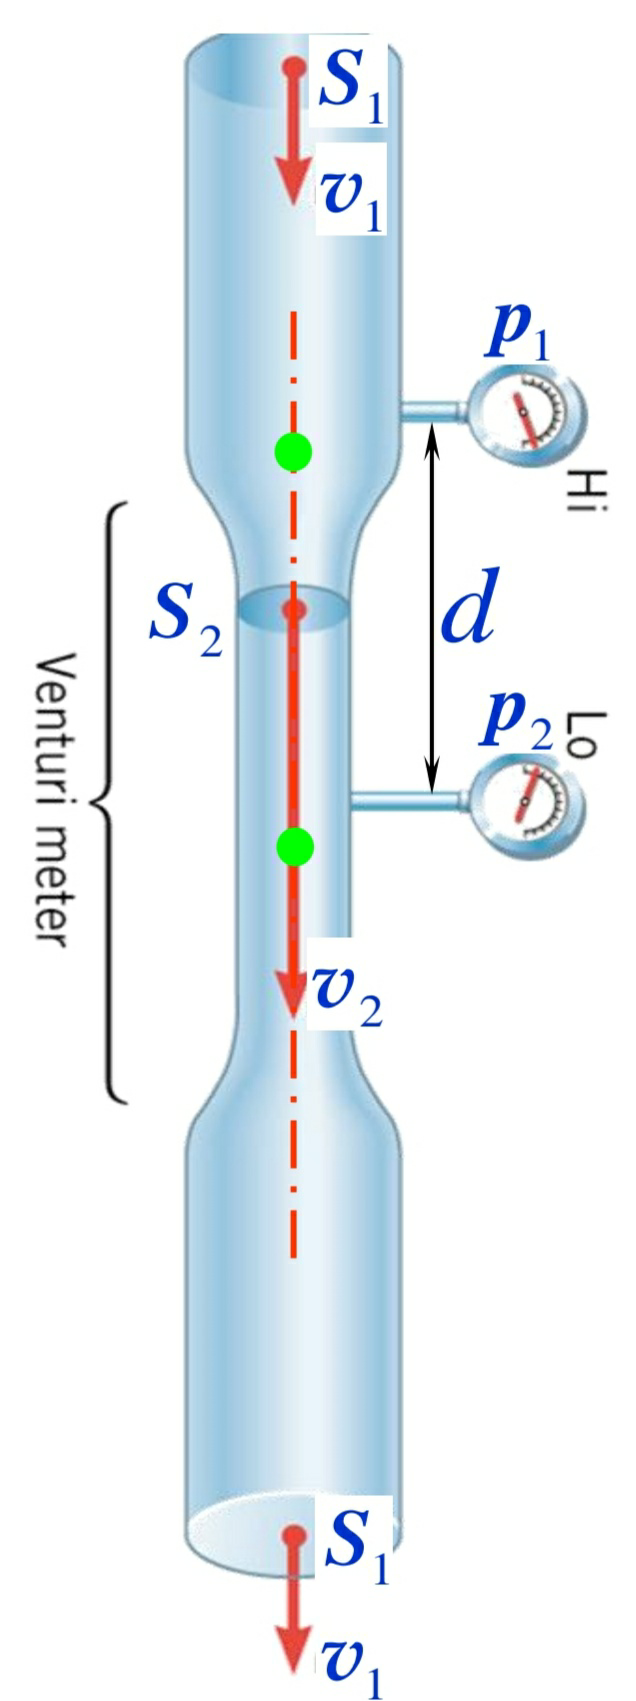
\includegraphics[scale=0.15]{Cf-pic (8).png}
    \end{center}
\end{multicols}
而空吸作用是利用增大流体流速而产生的对周围流体的吸入作用。在同一流管的稳定流动中,管径变细处流速增大而压强减小,当压强减小到低于周围流体的压强时,周围流体即向该处流入。如化油器、\textbf{真空抽机}、喷雾器等都是利用空吸作用原理设计制造的。

\subsubsection{例题}
如图所示为一装有喷嘴的水枪，在活塞上施加力F 时，水枪内部的水可以从喷嘴中喷出。设水枪的半径为R，喷嘴的半径为d。试求当施加力F 时，水的喷出速度是多少？
\begin{center}
    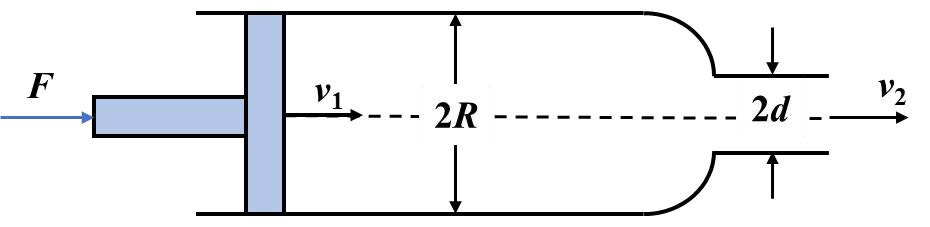
\includegraphics[scale=1]{Cf-ex.jpg}
\end{center}
\textbf{解：} 对于流线上两点，由伯努利方程：
\begin{equation}
     p_1+\frac{1}{2}\rho v_1^2=p_2+\frac{1}{2}\rho v_2^2
\end{equation} 
\begin{equation}
     p_0+\frac{F}{S_1}+\frac{1}{2}\rho v_1^2=p_0+\frac{1}{2}\rho v_2^2
\end{equation} 

而由连续性方程：
\begin{equation}
    v_1S_1=v_2S_2
\end{equation} 

由上两式，得：
\begin{equation}
     v=\sqrt{\frac{2 F}{\rho S_{1}\left(1-\frac{S_{2}^{2}}{S_{1}^{2}}\right)}}=\sqrt{\frac{2 F}{\rho \pi R^{2}\left(1-\frac{d^{4}}{R^{4}}\right)}}
\end{equation} 

\section{粘滞流体的运动}
所有流体在流动时具有 \textbf{粘滞性} ，因此会有能量的损耗。当 能量损耗 必须考虑时，将其作粘滞流体处理。
\begin{itemize}
         \item \textbf{层流} ：当流体流速较小时，保持分层流动，各流层之间只作相对滑动，彼此不相混合；
         \item \textbf{湍流} ：当粘滞流体流速较大时，容易产生径向流动（垂直于管轴方向的速度分量），各流层相互掺合，整个流体作无规则运动。
\end{itemize}

\subsection{雷诺数}
流体是作层流还是作湍流与一个无量纲的数$\rho vl/\eta$的大小有关，其称为雷诺数。对于圆形管道有$Re=\rho vd/\eta$.
\begin{center}
    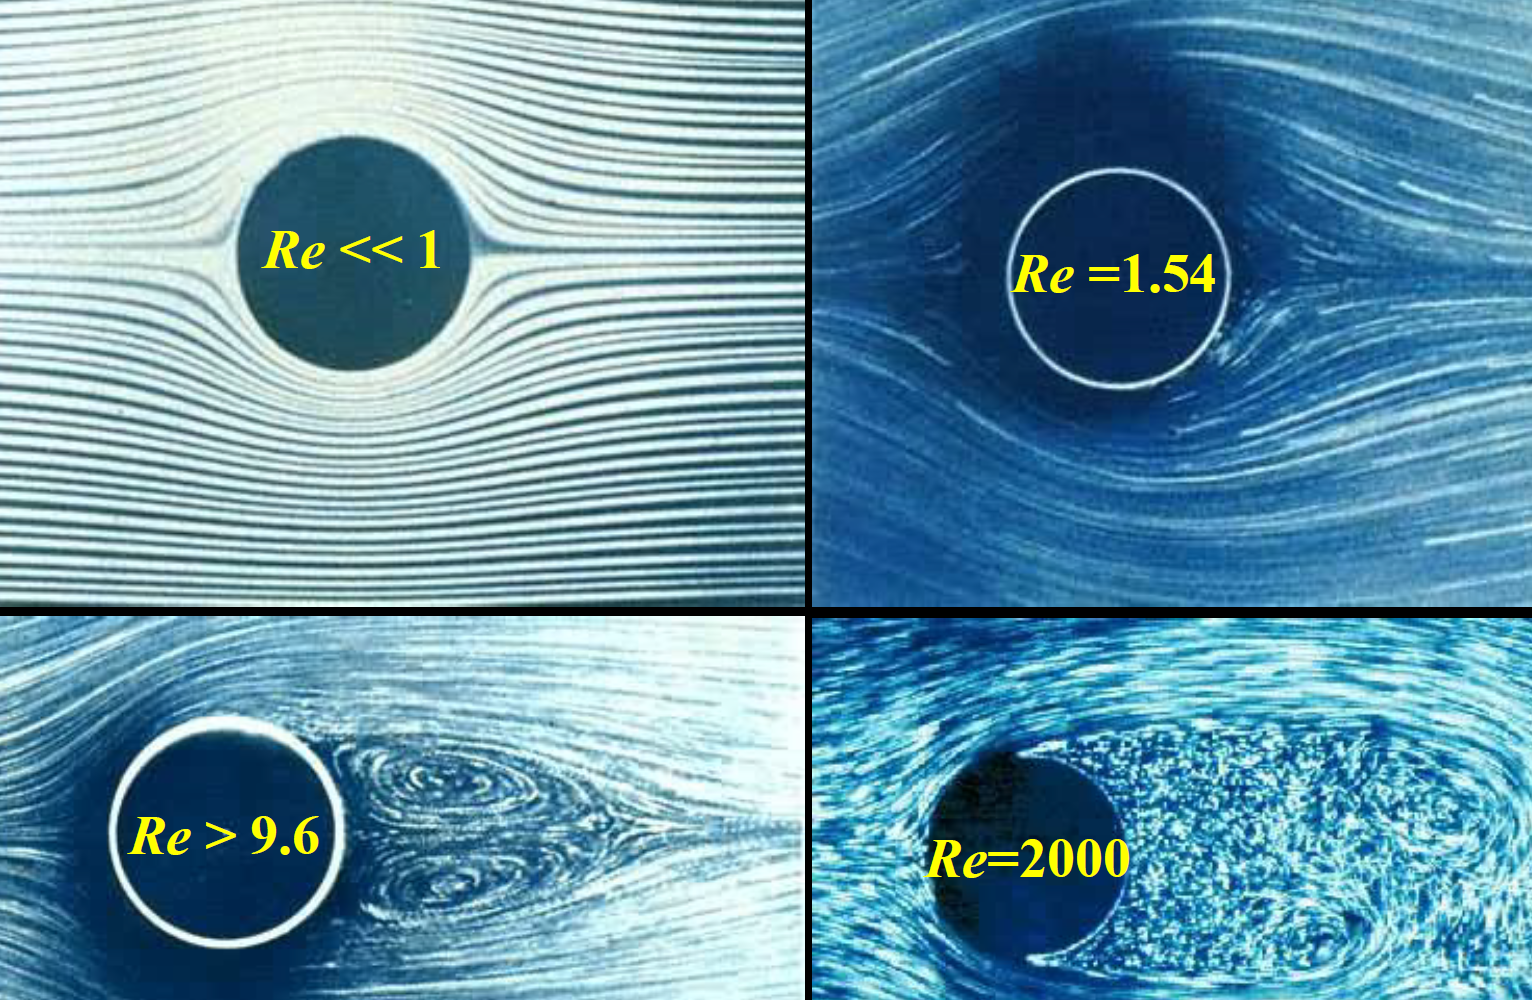
\includegraphics[scale=0.4]{Cf-pic (9).png}
\end{center}
\begin{itemize}
         \item \textbf{临界雷诺数}：流体由层流向湍流过渡的雷诺数；
         \item \textbf{湍流} ：当粘滞流体流速较大时，容易产生径向流动（垂直于管轴方向的速度分量），各流层相互掺合，整个流体作无规则运动。
\end{itemize}

\subsection{实际流体的粘滞定律}
在流动的粘滞流体中，如果相邻的流体质量元速度不同，它们之间存在着阻碍它们相对运动的力，称为粘滞阻力。
\begin{center}
    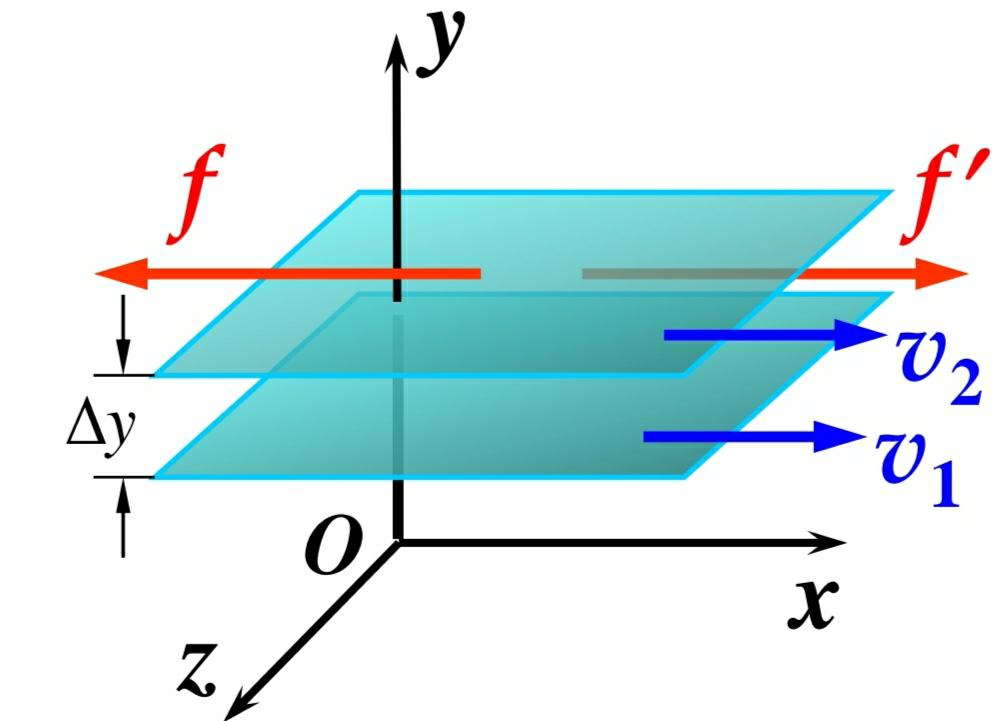
\includegraphics[scale=0.15]{Cf-pic (10).png}
\end{center}
1687年，牛顿发现作层流的粘滞流体中，流层间的粘滞阻力这种粘滞流体称为牛顿流体。
\begin{equation}
    f=-\eta \frac{dv}{dy}\Delta S
\end{equation}
比例系数η称为粘滞系数，与流体的属性和温度有关。
一般液体的η随T的升高而减小（主要取决于分子间吸引力）；气体的η随T的升高而增大（主要取决于热运动的动量交换）。

符合要求的粘滞流体称为牛顿流体。

实际流体稳定流动的伯努利方程也要加上单位体积粘滞力做功（负值）的项。

\subsection{泊肃叶公式等……}
\textit{直接的结论}: \textbf{$Q_V$与$R^4$成正比}，R对Q的影响非常大。
\begin{center}
    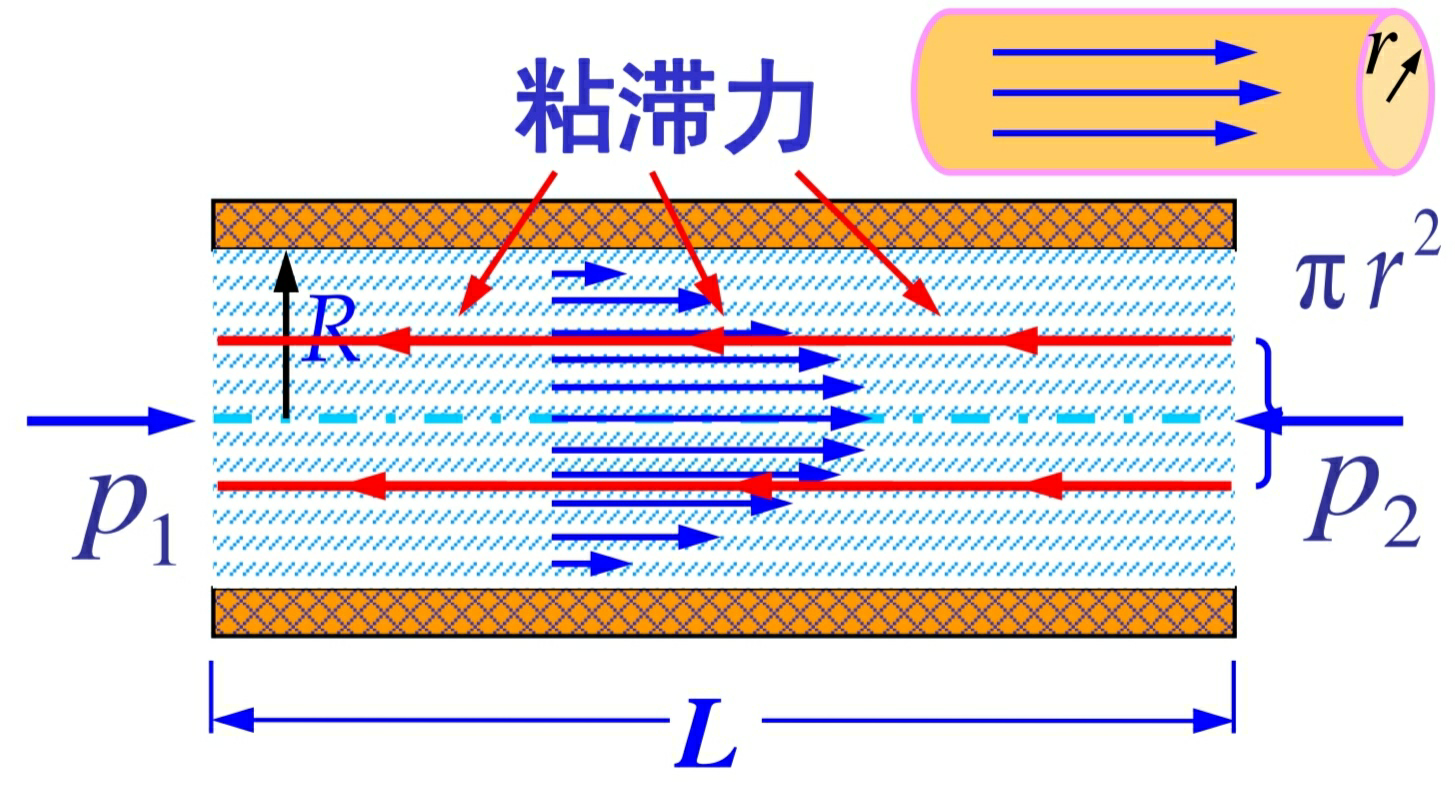
\includegraphics[scale=0.15]{Cf-pic (11).png}
\end{center}

由于每层的流速不同，要先求出速度随半径的变化规律。

粘滞阻力大小：
\begin{equation}
    f=-\eta \frac{dv}{dy}\Delta S
\end{equation}

稳定流动：
\begin{equation}
    (p_{1}-p_{2}) \pi r^{2}=-\eta · 2 \pi r L \frac{\mathrm{d} v}{\mathrm{~d} r}
\end{equation}
\begin{equation}
    -\int_{v}^{0} \mathrm{~d} v=\frac{p_{1}-p_{2}}{2 \eta L} \int_{r}^{R} r \mathrm{~d} r
\end{equation}
故，
\begin{equation}
v(r)=\frac{p_{1}-p_{2}}{4 \eta L}\left(R^{2}-r^{2}\right)
\end{equation}
所以，
\begin{equation}
    Q_{V} =2 \pi \int_{0}^{R} v(r) r \mathrm{~d} r =\frac{\pi}{8} \frac{p_{1}-p_{2}}{\eta L} R^{4}
\end{equation}
可用于测量粘度，另有斯托克斯公式\footnote{牛顿流体中作低速运动的小球所受阻力的大小$ f= 6 \pi \eta r v $}。
\begin{equation}
    \eta=\frac{2}{9} \frac{\rho-\rho_{0}}{v_{T}} g r^{2}
\end{equation}
~\\
~\\
~\\
~\\
~\\
~\\
~\\
~\\

流体力学是研究流体（包括气体和液体）运动规律的科学。它广泛应用于航空、航天、汽车、化工、生物医学工程、建筑环境与能源等领域。在实际应用中，我们需要结合具体情况来分析和运用流体力学的知识。

如果您希望对流体力学有更深入的了解或者想进一步探讨相关话题，请参加能源与动力工程学院开设的流体力学课程或查看专著。

% The End.